\clearpage
\section{Annex: Hardware Selection Details}
\label{sec:annex_hardware}

This annex preserves the detailed derivation of motor, battery, and voltage-sag trade-offs that informed the platform design. The main \autoref{sec:methodology} retains only the high-level reasoning.

\subsection{Thrust-to-Weight Ratio: Detailed Derivation}

\textbf{Definition and Target Range}

Thrust-to-weight (TWR) ratio expresses the total available thrust divided by drone mass. It directly determines hover efficiency and responsiveness. Industry guidelines establish a spectrum across applications.\cite{bershadsky2016propulsion}

\begin{table}[h]
\centering
\begin{tabular}{|c|c|c|c|}
\hline
\textbf{Application} & \textbf{TWR} & \textbf{Hover Throttle} & \textbf{Notes} \\
\hline
Aerial photography & 2:1 to 3:1 & 40--50\% & Stable, efficient \\
\hline
Research/cargo & 3:1 to 4:1 & 30--50\% & Responsive, good efficiency \\
\hline
Racing/freestyle & 5:1+ & 15--25\% & Aggressive maneuvers \\
\hline
\end{tabular}
\end{table}

\textbf{Why TWR Matters: Efficiency and Control Authority}

Motor efficiency does not follow a simple linear relationship with throttle percentage. Instead, efficiency curves show a \textbf{peak efficiency at mid-range throttle} (typically 40--70\%), with degradation at both very low and very high throttle levels.\cite{bershadsky2016propulsion} This is critical for autonomous drones.

If a drone hovers at 100\% throttle, it has zero authority to climb, stabilize, or reject wind gusts---any disturbance forces maximum output, leaving no control margin and risking loss of stability during maneuvers.\cite{bershadsky2016propulsion} Conversely, hovering at 40--50\% throttle reserves substantial available thrust for autonomous obstacle avoidance, gust rejection, and rapid maneuvers required during precision autonomous flight.\footnote{As recommended by commercial test platforms: \url{https://www.tytorobotics.com/blogs/articles/the-drone-design-loop-for-brushless-motors-and-propellers}}

\subsection{Motor Selection: EMAX ECOII 2004 1600KV}

\textbf{Why This Motor?}

The EMAX ECOII 2004 series is specified for 4--5 inch ultralight builds.\footnote{Product specifications available at: \url{https://emaxmodel.com/products/emax-eco-ii-series-2004-1600kv-2000kv-2400kv-3000kv-brushless-motor-for-rc-drone-fpv-racing}} The 2004 designation specifies stator dimensions: 20mm diameter and 4mm height.

Pilot testing of a similar 2004-series motor (T-Motor F2004 1700KV, comparable in stator dimensions) paired with 4-inch GF4023 propellers and a 6S battery demonstrated approximately 860 grams of static thrust per motor~\cite{bershadsky2016propulsion}\footnote{Product specifications available at: \url{https://drone24hours.com/products/t-motor-f2004-1700kv}}. With four motors, this yields combined thrust capacity of approximately 3,440 grams---establishing the system's TWR.

\textbf{TWR Calculation}:
\begin{itemize}
    \item Total available thrust: 3,440\,g (860\,g per motor $\times$ 4, estimated from published test data for a comparable T-Motor F2004 1700KV)
    \item Initial weight estimate: 800--1,000\,g $\rightarrow$ projected TWR of 4.30:1 to 3.44:1
    \item Design target weight: 1,200\,g $\rightarrow$ target TWR = 3,440 / 1,200 $\approx$ \textbf{2.87:1}
    \item Actual all-up weight (incl.\ PETG cage, bearing mechanism, wiring): $\sim$1,340\,g $\rightarrow$ actual TWR = 3,440 / 1,340 $\approx$ \textbf{2.57:1}
\end{itemize}

At 2.57:1, the design carries less thrust headroom than is typical for research-autonomy platforms---a direct consequence of the companion computer, protective cage, and bearing assembly, whose combined weight is unusual for a 4-inch airframe. Nevertheless, this ratio still provides sufficient thrust to arrest post-collision drift, and the motors operate near their efficiency peak at the resulting hover throttle of approximately 40\%.

\textbf{Understanding Motor Nomenclature}

The \textbf{2004 designation} specifies 20mm stator diameter and 4mm height. Larger stator diameters generate more torque but have slower transient response (RPM changes take longer to complete) compared to smaller-diameter motors.\cite{bershadsky2016propulsion} This trade-off is deliberate: at mid-throttle operation, the 2004's larger stator sustains higher efficiency than smaller, higher-KV alternatives that must spin faster to produce equivalent thrust. For autonomous flight requiring smooth, predictable thrust response, this characteristic is desirable.

The \textbf{1600 KV rating} indicates 1600 RPM per applied volt. This low-KV designation was selected specifically for the 6S battery voltage.

\subsection{Battery Selection: 6S LiPo}

\textbf{Why 6S and Not 4S?}

Battery voltage selection cascades through the entire drivetrain. The \textbf{6S (six-cell) LiPo pack} produces nominal voltage of 22.2V (6 cells \(\times\) 3.7V per cell).\cite{bershadsky2016propulsion} This voltage selection determines optimal motor KV and operating efficiency.

\textbf{1600 KV with 6S Battery:}
\begin{itemize}
    \item Theoretical no-load RPM: 1600 KV \(\times\) 22.2V = \textbf{35,520 RPM}\cite{bershadsky2016propulsion}
    \item Practical RPM under propeller load: \textasciitilde24,000--28,000 RPM (typically 70--80\% of theoretical no-load speed due to air resistance and propeller drag)\cite{bershadsky2016propulsion}
    \item This range is optimal for 4-inch propellers, avoiding excessive tip speeds that reduce aerodynamic efficiency
\end{itemize}

\textbf{Higher voltage = less current for equivalent thrust.} When motors operate on 4S (\textasciitilde14.8V nominal), they require significantly higher current draw to achieve the same thrust.\cite{bershadsky2016propulsion} Higher current increases internal losses in battery, ESCs, and motor windings---manifesting as excess heat and reduced flight time. 6S draws proportionally less current for equivalent thrust, keeping system temperature lower. This follows directly from the power-voltage-current relationship ($P = VI$): for a fixed power demand, raising the bus voltage reduces the required current, and resistive copper losses ($I^2R$) in the windings and controllers decrease quadratically.\cite{hughes2013electric}

\subsection{Voltage Sag: Detailed Mechanism}

\textbf{What is Voltage Sag and Why It Matters}

Voltage sag refers to the \textbf{temporary voltage drop that occurs during high-current discharge events}. This drop is caused by battery internal resistance (IR). Ohm's Law describes this relationship: \textbf{Voltage Drop = Current \(\times\) Internal Resistance}.\cite{bershadsky2016propulsion}

Every LiPo battery contains internal resistance---even high-quality cells. When you demand high current from the battery (e.g., during rapid acceleration), that current flowing through internal resistance creates a voltage drop.\cite{bershadsky2016propulsion} For example:

\begin{itemize}
    \item A 4S battery (14.8V nominal) with typical internal resistance might sag from 14.8V down to \textbf{10.2V} during peak acceleration
    \item A 6S battery (22.2V nominal) with equivalent quality, under the same peak current draw, experiences proportionally less sag (from 22.2V down to \textasciitilde16.5V)\cite{bershadsky2016propulsion}
\end{itemize}

The absolute sag magnitude (difference in volts) may be similar between 4S and 6S. \textbf{But the percentage impact is vastly different:}

\begin{itemize}
    \item 4S sag example: 14.8V \(\to\) 10.2V is a \textbf{31\% voltage loss}
    \item 6S sag example: 22.2V \(\to\) 16.5V is only a \textbf{26\% voltage loss}
\end{itemize}

\textbf{Why This Matters for Autonomous Flight Controllers}

The Pixhawk 6C relies on stable voltage to maintain consistent motor response during rapid maneuvering. The flight controller sends throttle commands expecting motors to accelerate at a predictable rate. \textbf{Excessive voltage sag introduces latency between commanded acceleration and actual motor output.} The causal chain:

\begin{enumerate}
    \item Flight controller commands 70\% throttle for obstacle avoidance maneuver
    \item Motor voltage sags unexpectedly from 22V to 16V due to high current draw
    \item Motor RPM drops below what the controller expected
    \item Actual thrust output is lower than the controller's state estimator predicted
    \item The control loop detects the mismatch and must recalculate---introducing lag
\end{enumerate}

During high-speed autonomous maneuvers, this lag degrades control stability and can risk uncommanded behavior. Higher baseline voltage (6S) provides a larger voltage margin, reducing the percentage impact of sag on motor performance.\cite{bershadsky2016propulsion}

\textbf{6S Enables Efficient Hover at Higher Throttle Margin}

Since 6S provides higher baseline voltage, the motor's hover throttle point is positioned differently on the efficiency curve compared to 4S. Hover throttle percentage depends on specific motor and load characteristics---\textbf{there is no direct proportionality between voltage and hover throttle}. However, empirical trends confirm that 6S configurations maintain superior efficiency up to approximately 45\% throttle before the efficiency curves converge.\cite{hughes2013electric}

The 1600KV motor on 6S should hover at approximately \textbf{40\% throttle} based on the actual drone weight and motor thrust.\cite{bershadsky2016propulsion} This operating point sits within the motor's efficiency band and reserves approximately 60\% available thrust for maneuvers and environmental disturbances.

\subsection{System Integration: How Components Work Together}

This configuration is tightly coupled---changing any single parameter cascades inefficiencies throughout the system:

\begin{table}[h]
\centering
\begin{tabular}{|c|c|p{5cm}|}
\hline
\textbf{Parameter} & \textbf{Design} & \textbf{Rationale} \\
\hline
Frame size & 4-inch wheelbase & Pixhawk 6C form factor (84.8 \(\times\) 44 \(\times\) 12.4 mm) + indoor flight compliance \\
\hline
Motor KV & 1600 KV & Produces 24,000--28,000 RPM under load on 6S; optimal for 4-inch propellers\cite{bershadsky2016propulsion} \\
\hline
Battery voltage & 6S (22.2V nominal) & Reduces voltage sag percentage impact; improves efficiency at cruise throttle \\
\hline
Hover throttle & \textasciitilde40\% & Operates within motor efficiency band; reserves $\sim$60\% thrust headroom\cite{bershadsky2016propulsion} \\
\hline
TWR & 2.57:1 & Actual TWR with final assembly weight of $\sim$1,340\,g; target was 2.87:1 at 1,200\,g \\
\hline
\end{tabular}
\end{table}

If switched to 4S battery, for example, lower-KV motors would be needed (e.g., 1100KV) to maintain similar RPM. But lower-KV motors produce less torque, potentially requiring larger propellers or higher current draw---both of which degrade efficiency. Every selection interconnects. The component choices represent a validated system point.

\subsection{Supporting Plot: Motor Command Saturation During Impact}

\autoref{fig:allocator_saturation} presents the distribution of motor command saturation durations for both cage configurations. The plot shows the time during which the flight controller's motor mixer commanded ≥99.9\% of full output range in the first second after impact, providing direct evidence for the allocator saturation metrics discussed in \autoref{sec:impact_acceleration_vibrations}.

\begin{figure}[htbp]
    \centering
    \includegraphics[width=0.75\textwidth]{plots/Allocator Saturation Duration.png}
    \caption{Motor command saturation duration after impact for both cage configurations. Saturation is defined as motor command ≥99.9\% of the full output range.}
    \label{fig:allocator_saturation}
\end{figure}

\clearpage
\subsection{CAD Assembly Drawing}

\begin{landscape}
\begin{figure}[htbp]
    \centering
    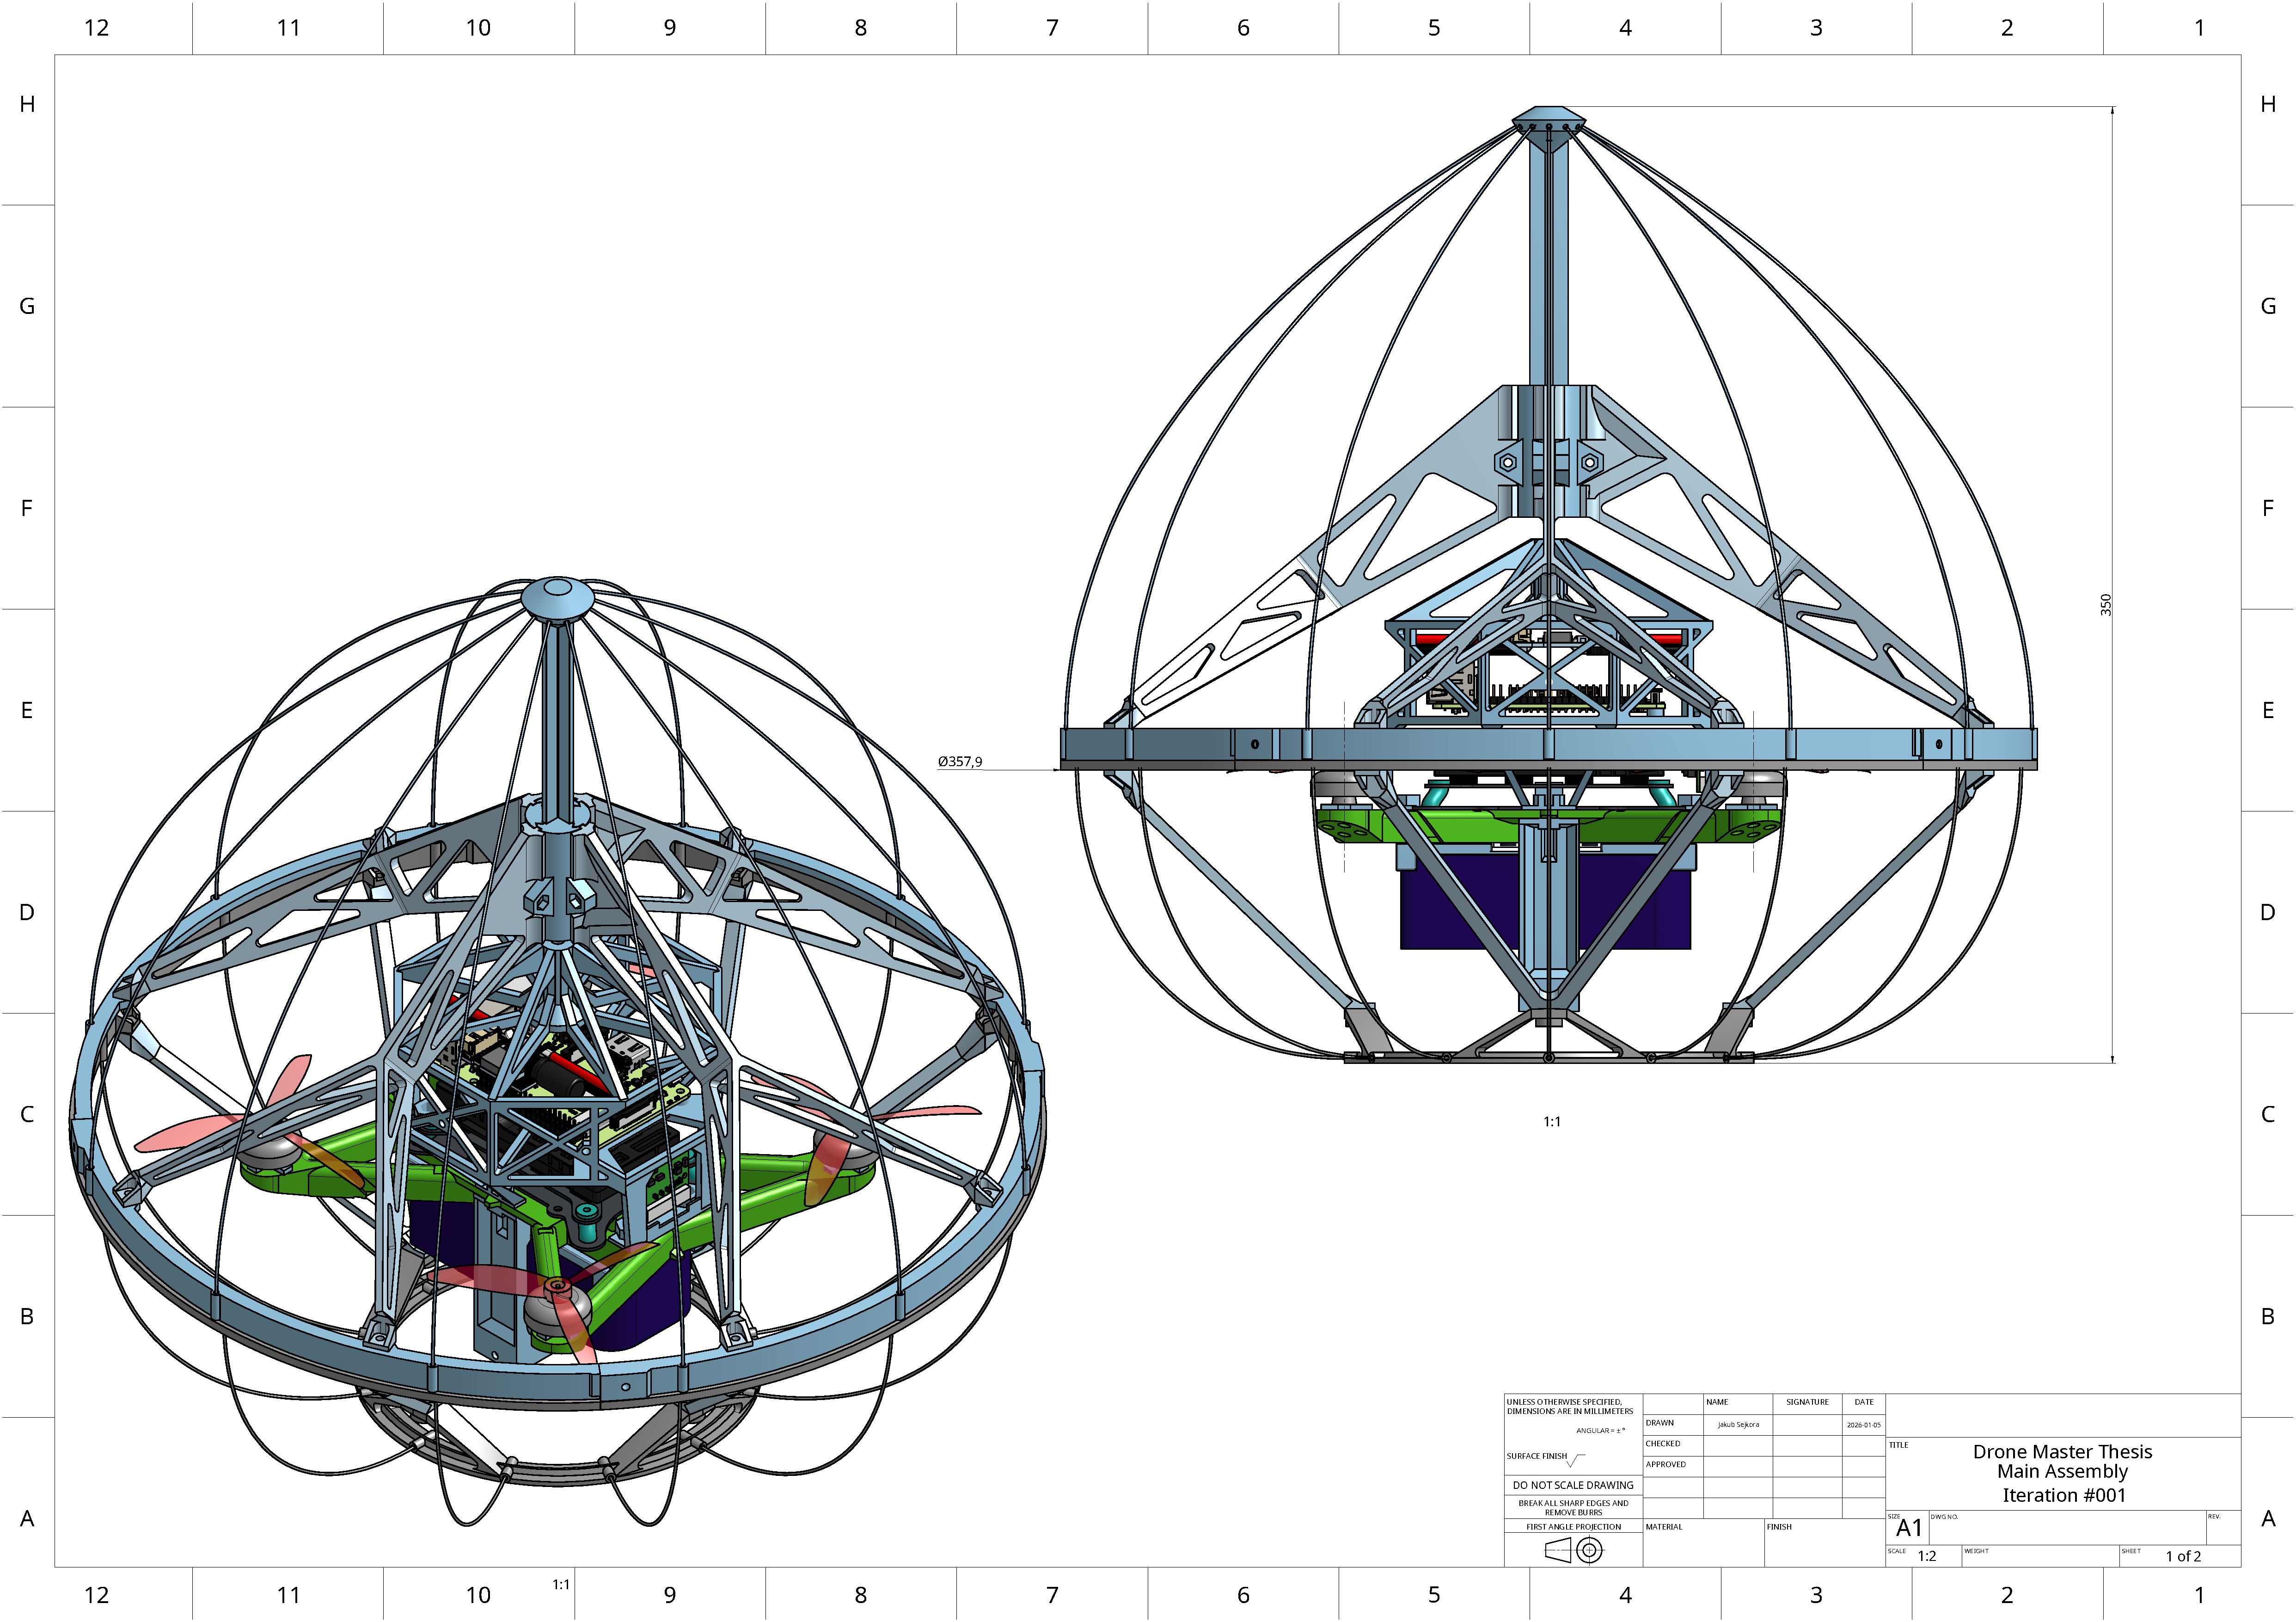
\includegraphics[width=\textwidth,height=0.90\textheight,keepaspectratio]{diagrams/drone_dwg.pdf}
    \caption{Full drone assembly drawing (sheet 1 of 2). The A1 original has been scaled to fit A4 page dimensions.}
    \label{fig:cad_assembly}
\end{figure}
\end{landscape}

\clearpage
\begin{center}
    \vspace*{4cm}
    {\LARGE\textbf{3D CAD Model}} \\[2em]
    \qrcode[height=4cm]{https://cad.onshape.com/documents/7cbebd1596e6b9c6c98f0e3f/w/5e6908f6b6eb3e1d2b683876/e/866a8eb8a37ae0706272cbd1?renderMode=0&uiState=6a4263881140b20f69c49cb9} \\[1em]
    {\footnotesize\url{https://cad.onshape.com/documents/7cbebd1596e6b9c6c98f0e3f/w/5e6908f6b6eb3e1d2b683876/e/866a8eb8a37ae0706272cbd1?renderMode=0\&uiState=6a4263881140b20f69c49cb9}} \\[2em]
    \large{The complete drone assembly CAD model, including the frame, protective cage, and all mounted components. This OnShape document served as the primary mechanical reference throughout the design, manufacturing, and assembly phases.}
    \vfill
\end{center}

\endinput
